\chapter{Related Work}
\label{chapter:related-work}

%% \cite{Kadiri2015} importance of technical analysis. questionnaire and an
%% interview survey to traders perceived importance of chartist/technical
%% interpretation, technical analysis is as used as fundamental, the shorter the
%% forecasting horizon, the more important technical analysis is. chartism may have
%% increased over the last decade. psychological motives by using chartism

%% Taylor, Mark and Allen, Helen \cite{Fund1992} technical analysis
%% importance. questionnaire survey. at least 90 per cent of respondents place some
%% weight on this form of non-fundamental analysis when forming views at one or
%% more time horizons. tech and fund are complementary. tech may be
%% sulf-fulfilling.

%% it could be a self-fulfilling prophecy
%% \cite{Salganik2008} self-fulfilling prophecy. false-popularity became real over
%% time (songs). the real songs recovered their popularity in the long run.

%% we can use tech ind to curve-fitting to forecast
%% In several efforts, researchers create regression models using technical or
%% fundamental indicators as training datasets. Examples of regression techniques
%% are autoregression \cite{burg1968new}, symbolic regression
%% \cite{billard2002symbolic}, and linear regression \cite{kutner2004applied}.

%% we can use tech ind to interpret the market
%% \cite{Ijegwa2014} interpretation. decisions. fuzzy inference to stock market,
%% using four indicators. deal with probability. The four technical indicators are
%% the Moving Average Convergence/Divergence (MACD), Relative Strength Index (RSI),
%% Stochastic Oscillator (SO) and On-Balance Volume (OBV). Fuzzy manually
%% designed. The result is a recommendation to buy, sell or hold. Data two nigerian
%% banks. Two months of data.

%% other techniques to forecast
%% \cite{Cai2013} forecast. fuzzy time series and genetic algorithm. uses GA to
%% optimize. TAIEX is used as data set. they get a low error.

%% a popular choice is neural networks
%% \cite{Castillo2001} neural networks for simulating and predicting financial
%% markets. comparison against fuzzy logic models and against statistical
%% model. tomato and green onion markets in the us.

%% \cite{melin2007hybrid} neural network simulate and predict financial
%% market. it's the same as Castillo2001.

%% \cite{Connor2005} uses neural network. using external indicators (commodity
%% prices exchange rates) in predictinng dow jones.

%% one last choice is multi-agents
%% \cite{Gamil2007} multi-agent, fuzzy logic decision support system. stock
%% market. help to take the correct buy/sell/hold decisions. fuzzy tuning
%% methodology used to enhance the accuracy of the decisions. genetic algorithm to
%% optimize. NASDAQ dataset.

This Chapter focuses on showcasing a series of works that should help the reader
understand what is the state of the different parts that compose the proposed
method presented in Chapter \ref{chapter:proposed-method}.

\section{Financial Forecasting}
\label{section:financial-forecasting}

Determining if a financial market should be traded is a process that can be
approached in different ways. For example, a straightforward method is to
analyze the financial health of a company to infer if it would be a good idea to
buy stock from it. This approach is known as fundamental analysis
\cite{Martinez-Jaramillo2009} and it is often contrasted to technical analysis,
which focuses on the analysis of historical prices of a financial market to
arrive at such inferences. Technical analysis involves any process that uses as
input the market prices and the output can usually be plotted along with the
market prices \cite{Achelis2000}. These processes are known as technical
indicators, which often focus on providing the chartist with information about a
market that would be difficult to infer by only looking at the raw price data.

Although some studies have suggested that technical analysis works because it is
``self-fulfilling prophecy'' \cite{Salganik2008} \cite{Fund1992}, other studies
also suggest that its usefulness in market forecasting is important
\cite{Kadiri2015} \cite{Fund1992}.

This thesis suggests that a financial market's data should be preprocessed
before being used as input for a modelling algorithm. The preprocessing
algorithm showcased in the proposed method is very similar in nature to what a
technical indicator is. Furthermore, the preprocessing algorithm is based on the
idea of an existing technical indicator known as Fibonacci retracements. It can
also be noted that the preprocessing algorithm presented in this thesis shares
some similarity to fuzzy time series \cite{Cai2013}, as the price areas that it
outputs can be seen as price levels associated with a level of uncertainty.

Technical indicators can be used to forecast a market's prices, such as in the
case of candlestick patterns \cite{Nison1991} or linear regression
\cite{kutner2004applied} which, although it is used in other contexts involving
time series, could be considered a technical indicator if used to forecast a
financial market. One can add an extra layer in the forecasting process and use
the outputs from the technical indicators as inputs to another algorithm. For
example, Ijegwa et al. \cite{Ijegwa2014} use four technical indicators as the
inputs for a fuzzy system that estimates the probability of a market's price
going up or down. This approach is similar to the one proposed in this thesis,
as the preprocessing algorithm is based on a technical indicator and it is used
as input for fuzzy systems that function as the rule systems for the agents in a
multi-agent system.

Arguably one of the most common methods used to forecast financial markets is
neural networks. For example, Castillo and Melin \cite{Castillo2001}
\cite{melin2007hybrid} use neural networks to forecast the prices of tomato and
green onion markets in the United States. One can also combine the idea of
preprocessing a market's prices using technical indicators and then use these
outputs as the inputs for a neural network, as in the work by O'Connor
\cite{Connor2005}. Neural networks were the first candidate for modelling the
agents' rules in the proposed method, as it is a common technique as described
in \cite{Grothmann2002}, but the use of fuzzy systems for this purpose seemed as
a better approach by the author of this thesis, as fuzzy systems are more
interpretable than the models generated by neural networks. As an example of a
similar approach to the aforementioned one, Gamil et al. \cite{Gamil2007} create
a multi-agent system that is tuned using a fuzzy system in order to create a
simulation of the NASDAQ index.

\section{Interpretation of Financial Markets}
\label{section:interpretation-of-financial-markets}

Technical indicators can be used to interpret the price data of financial
markets. For example, Wilder's Parabolic SAR can be used to determine if a
market has shifted its trend \cite{Wilder1978}. In the case of the proposed
method's preprocessing algorithm, its plots can be used to determine possible
price stagnation or bouncing areas.

%% market interpretability help choosing stocks
\cite{Brown2013} interpretation. niche genetic algorithm to select stocks from
dow jones. uses another algorithm to forecast markets. then chooses the best.

The work by Brown, Pelosi and Dirska uses a Niche Genetic Algorithm called
Dynamic-radius Species-conserving Genetic Algorithm (DSGA) to select stocks to
purchase from the Dow Jones Index.

%% decision support systems
\cite{Keen1980} general theory about decision support systems.

%% example of a DSS
\cite{Tsang2004} interpretability. Evolutionary Dynamic Data Investment
Evaluator (EDDIE) is a genetic programming (GP)-based decision support tool for
financial forecasting. It serves to improve the productivity of experts in
searching the space of decision trees, with the aim to improve the odds in its
user’s favour.

\cite{tsang1998eddie} EDDIE has been applied to horse racing and achieved
outstanding results. When experimented on 180 handicap races (real data) in the
UK, it out-performed other common strategies. The idea was then extended to
financial forecasting. When tested on historical S&P-500 data EDDIE achieved a
respectable annual rate of return over a three and a half year period.

%% further studies about DSS
\cite{Sprague1980} DSS. examines people using it, the roles and types of people
using the DSS. outlines issues in their use.

%% we can use tech ind to interpret the market
\cite{Ijegwa2014} interpretation. decisions. fuzzy inference to stock market,
using four indicators. deal with probability. The four technical indicators are
the Moving Average Convergence/Divergence (MACD), Relative Strength Index (RSI),
Stochastic Oscillator (SO) and On-Balance Volume (OBV). Fuzzy manually
designed. The result is a recommendation to buy, sell or hold. Data two nigerian
banks. Two months of data.

%% interpret using candlesticks
\cite{Nison1991} general theory about japanese candlesticks and patterns.

%% wilder's they interpret different aspects
\cite{Wilder1978} theory about his technical indicators.

%% how volume can be used to interpret the market
\cite{Blume1994} agents learning process. technical analysis. investigate the
informational role of volume and its applicability for technical
analysis. traders receive signals with differing quality. We show how volume,
information precision, and price movements relate, and demonstrate how sequences
of volume and prices can be informative.

%% automatic pattern finding
\cite{Lo2000} technical analysis. automatic approach to technical pattern
recognition using kernel regression. u.s. stocks to evaluate the effectiviness
of tech analysis. they do provide incremental information and may have some
practical value.

%% finding tech rules
\cite{Neely1997} genetic programming to find technical trading
rules. Bootstrapping results on the dollar/Deutsche mark indicate that the
trading rules detect patterns in the data that are not captured by standard
statistical models.

%% tech analysis can be used to reduce noise. here's another work:
The work by Lu, Lee, and Chiu \cite{Lu2009} point out the complexity of
financial time-series. They note its noisy nature and propose a technique to
reduce this noise based in a two-stage modeling approach using Independent
Component Analysis (ICA) and Support Vector Regression (SVR). Their approach
first uses ICA for generating independent components to identify and remove
those containing the noise, then the remaining components are used to
reconstruct the forecasting variables which now contain less noise and are the
input of the SVR forecasting model.

\section{Multi-agent Systems}
\label{section:multi-agent-systems}
% agents can also be used to generate interpretations
% basic concepts
\cite{Grothmann2002} general theory about multi agent systems in market
modelling using neural networks.  \cite{Lebaron2001} a builder's guide to agent
based financial markets.

As a final mention, Samanidou, et. al. \cite{Samanidou_2007}, provides the
reader a very comprehensive overview of Agent-based Modeling, where different
techniques to perform this kind of models are discussed.

The authors of this work gained useful knowledge about multi-agent system from
two theses. The first one is the work from Grothmann \cite{Grothmann2002},
``Multi-agent Market Modeling based on Neural Networks.'' This work served as
inspiration for the architecture of the Proposed Method. The second thesis is
\cite{Boer-Sorban2008}'s ``Agent-Based Simulation of Financial Markets,'' which
gave an overview of approaches to describe and understand financial market's
dynamics, and motivated the authors of this work to use the approach of
Agent-based Computation to perform financial forecast.

%% introduction
\cite{Shoham2009} I use this architecture.

%% some microscopic models
\cite{Bundesbank2007} agents. several microscopic (“agent-based”) models of
financial markets which have been studied by economists and physi- cists over
the last decade: Kim-Markowitz, Levy-Levy-Solomon, Cont- Bouchaud,
Solomon-Weisbuch, Lux-Marchesi, Donangelo-Sneppen and Solomon-Levy-Huang. aim is
to reproduce (and, thereby, provide possible explana- tions) for the bubbles and
crashes seen in certain histori- cal episodes.

%% one agent per strategy, similar than previous
\cite{Sherstov2005} three autonomous stock trading agents. within the framework
of the Penn Exchange Simulator (PXS), a novel stock-trading simulator. The three
approaches presented take inspiration from reinforcement learning, myopic
trading using regression-based price prediction, and market making. The
market-making strategy was the winner in the fall 2003 PLAT live competition.

%% simulation
Kendall and Su \cite{Kendall2003} use a multi-agent system to simulate stock
markets within which stock traders are modeled as heterogeneous adaptive
artificial agents. On average, 80\% of the artificial stock traders were able to
trade using successful trading strategies which brings the investors higher
returns compared to a simple buy-and-hold strategy.

%% population of agents, evolved. similar to proposed method
\cite{Chen2001} close to proposed method. agents. population of
agents. consideration trader's search behavior. evolve population using
GP. connect search density to psychological factors such as peer pressure.

\section{Evolutionary Algorithms}
\label{section:evolutionary-algorithms}

%% different evolutionary algorithms
\cite{Back2008} compared in this article: evolution strategies (ESs),
evolutionary programming (EP), and genetic algorithms (GAs).

%% variations of GA
\cite{Harik1999} — a custom. compact genetic algorithm. It processes each gene
independently and requires less memory than the simple GA. efficiency.

%% alternatives considered
\cite{Eberhart2002} pso first paper.

\cite{Price1997} Differential evolution paper.

%% practical example
Thrift \cite{Thrift1991} explores a nowadays widely used technique which
involves the use of a Genetic Algorithm (GA) to discover the parameters of the
Membership Functions (MF) in a Fuzzy Inference System to obtain a better
performance. Homaifar and McCormick \cite{Homaifar1995} go further and use GA to
simultaneously design the MF and the rule sets for fuzzy logic controllers.

%% basic concepts about GA and variations.
%% finish stating we use this
\cite{Whitley1994} tutorial for genetic algorithm, parallel island models,
parallel cellular genetic algorithms. theoretical foundations of genetic
algorithms.

\section{Fuzzy Systems}
\label{section:fuzzy-systems}

\cite{Zadeh1965} zadeh fuzzy sets.

\cite{Mamdani1975} Mamdani paper.

\cite{Takagi1985} Sugeno paper.

% comparison against type-2

\cite{Mendel2002} Type-2 introduction \cite{Mendel2006} type-2 interval theory
\cite{Liang2000} Type-2 interval theory \cite{Karnik2001} Centroid of a type-2
fuzzy set.

\cite{Pedrycz1998} shadowed sets. enhancing interpretation of results obtained
therein. it is demonstrated how fuzzy sets can induce shadowed sets.

%% ifis
\cite{Atanassov1986} intuitionistic fuzzy sets paper.  \cite{Atanassov2003}
Intuitionistic fuzzy sets: past, present and future.


%% implementations
Wagner presents a robust implementation of FISs developed in Java in
\cite{Wagner2013}. The authors of the present work have used this particular
toolkit for comparisons in the capabilities of the IFIS to model uncertainty
against type-1 FISs and interval type-2 FISs in
\cite{Hernandez-Aguila2016}. Although the toolkit does not provide many tools
for representing a FIS graphically or for interacting with one, the
implementation provides libraries for building type-1, interval type-2, and
generalized type-2 fuzzy systems.

The work by Castro et al. \cite{castro2007interval} provides similar
capabilities as the work by Wagner, but in this case it is an implementation in
Matlab. A direct disadvantage of using this programming language is that Matlab
is not a free nor open source software.  Nevertheless, the language is still
widely used in the scientific community. Furthermore, this implementation
follows an interface similar to the one provided by Matlab's fuzzy logic
toolbox, and provides more robust graphical implementations than the current
version of Wagner's toolkit.

% fuzzy software
\cite{Wagner2013} java based type-2.

\cite{castro2007interval} Ramon toolbox.

\cite{Hernandez-aguila2016} My Proposal \cite{Hernandez-Aguila2017} My
Implementation

% mention my works, the proposal and the implementation

%% imembership function design
The most common approach to graphically representing an IFS is by
lattices. Examples of this type of representation can be found in the works by
I. Despi et al. \cite{Despi2013}, and G. Deschrijver et
al. \cite{Deschrijver2004}. This is a popular approach to graphically represent
an IFS as it enables more compact and concise mathematical expressions. Another
representation that is suitable for mathematical processes is that of a matrix,
and is discussed in detail in the works by R. Parvathi et
al. \cite{Parvathi2014}, G. Çuvalcioglu et al. \cite{Yilmaz2015}, and S. Yilmaz
et al. \cite{Yilmaz2015a}.

IFSs that are graphically represented like membership functions are usually
represented in Mamdani FISs, and some example works are the ones by
K. T. Atanassov \cite{Atanassov1986}, and H. Davarzani and M. A. Khorheh
\cite{Davarzani2013}. This notation can be suitable for representing an
architecture of an IFIS, but if the plot is in black and white, or in greyscale,
the reader can get confused by the membership and non-membership plots. This
problem can be alleviated by plotting the membership and non-membership
functions in separate plots, as in the works by O. Castillo et
al. \cite{castillo2007intuitionistic}, and M. Akram et al. \cite{Akram2014}.

There are several other graphical representations of IFSs, such as by radar
charts, as in the work by V. Atanassova \cite{Atanassova2010}, and by
geometrical representations, orthogonal projections and three-dimensional
representations, as can be found in the work by E Szmidt and J. Kacprzyk
\cite{Szmidt2000}.

Some applications of IFSs in the area of medical sciences can be found in the
works by E. Szmidt and J. Kacprzyk \cite{Szmidt2001}, C. M. Own \cite{Own2009},
and D. D. Chakarska and L. S. Antonov \cite{Antonov1995}. In the area of group
decision making, we have an example in the work by Z. Xu \cite{Xu2007}. IFSs
have also been used in word recognition, in the area of artificial vision, as in
the example work of L. Baccour et al. \cite{Baccour2008}.

This work proposes that IFSs, in a Mamdani IFIS, should follow an approach
similar to that found in the work by K. T. Atanassov \cite{Atanassov2003}, where
the membership is plotted as is commonly done in a traditional FIS, but the
non-membership function should be plotted as 1-υA. The reason behind this
decision is that the non-membership function should be easily differentiated
from the membership function, while seeing both functions in the same plot. An
implementation of an IFIS that uses this approach for representing IFSs for a
Mamdani IFIS can be found in the work by A. Hernandez-Aguila and
M. Garcia-Valdez \cite{Hernandez-aguila}.

In Figure \ref{figure:traditional-set-as-ifs}, one can see how a traditional
fuzzy set can be constructed using the proposed approach. A Gaussian membership
function with mean of 50 and a standard deviation of 15 is depicted.

\begin{figure}
\caption{A traditional fuzzy set represented as an intuitionistic fuzzy set}
\centering 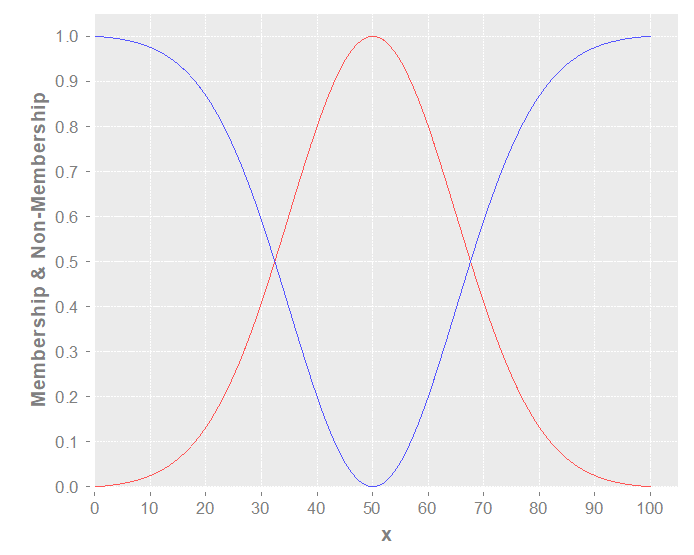
\includegraphics[width=0.7\textwidth]{img/traditional-set-as-ifs.png}
\label{figure:traditional-set-as-ifs}
\end{figure}

Figure \ref{figure:example-of-ifs} is the first case of an IFS that cannot be
considered a tradi-tional fuzzy set. The red line represents the membership
function, while the blue line represents the non-membership function. As can be
seen, the Gaussian membership function does not have a kernel, meaning that its
highest valued member does not equal to 1. In this case, its highest valued
member equals to 0.7, and for the non-membership function, its highest valued
member equals to 0.3. The Gaussian membership function is constructed with a
mean of 50 and a standard deviation of 15. For the non-membership function, it
is con-structed with a mean of 30 and standard deviation of 30.

\begin{figure}
\caption{Representation of an intuitionistic fuzzy set} \centering
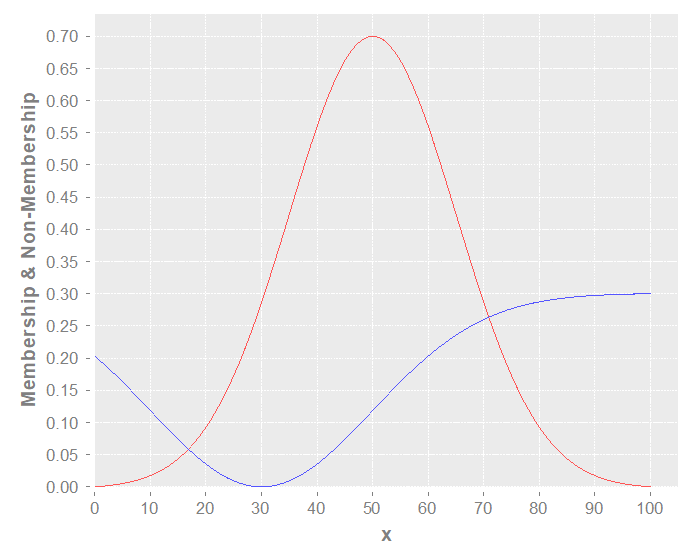
\includegraphics[width=0.7\textwidth]{img/example-of-ifs.png}
\label{figure:example-of-ifs}
\end{figure}
